\documentclass{article}
\usepackage{tikz}
\usetikzlibrary{calc,fadings,decorations.pathreplacing,backgrounds}
\usepackage{verbatim}
%% helper macros
\newcommand\pgfmathsinandcos[3]{%
  \pgfmathsetmacro#1{sin(#3)}%
  \pgfmathsetmacro#2{cos(#3)}%
}
\newcommand\LongitudePlane[3][current plane]{%
  \pgfmathsinandcos\sinEl\cosEl{#2} % elevation
  \pgfmathsinandcos\sint\cost{#3} % azimuth
  \tikzset{#1/.estyle={cm={\cost,\sint*\sinEl,0,\cosEl,(0,0)}}}
}
\newcommand\LatitudePlane[3][current plane]{%
  \pgfmathsinandcos\sinEl\cosEl{#2} % elevation
  \pgfmathsinandcos\sint\cost{#3} % latitude
  \pgfmathsetmacro\yshift{\cosEl*\sint}
  \tikzset{#1/.estyle={cm={\cost,0,0,\cost*\sinEl,(0,\yshift)}}} %
}
\newcommand\DrawLongitudeCircle[2][4]{
  \LongitudePlane{\angEl}{#2}
  \tikzset{current plane/.prefix style={scale=#1}}
   % angle of "visibility"
  \pgfmathsetmacro\angVis{atan(sin(#2)*cos(\angEl)/sin(\angEl))} %
  \draw[current plane] (\angVis:1) arc (\angVis:\angVis+180:1);
  \draw[current plane,dashed] (\angVis-180:1) arc (\angVis-180:\angVis:1);
}
\newcommand\DrawLatitudeCircle[2][5]{
  \LatitudePlane{\angEl}{#2}
  \tikzset{current plane/.prefix style={scale=#1}}
  \pgfmathsetmacro\sinVis{sin(#2)/cos(#2)*sin(\angEl)/cos(\angEl)}
  % angle of "visibility"
  \pgfmathsetmacro\angVis{asin(min(1,max(\sinVis,-1)))}
  \draw[current plane] (\angVis:1) arc (\angVis:-\angVis-180:1);
  \draw[current plane,dashed] (180-\angVis:1) arc (180-\angVis:\angVis:1);
}

%% document-wide tikz options and styles

\tikzset{%
  >=latex, % option for nice arrows
  inner sep=0pt,%
  outer sep=2pt,%
  mark coordinate/.style={inner sep=0pt,outer sep=0pt,minimum size=4pt,
  fill=black,circle}%
}

\begin{document}
\begin{tikzpicture}[rotate=-23.5] % "THE GLOBE" showcase


    \def\R{2} % sphere radius
    \def\angEl{5} % elevation angle
    \def\angAz{105} % azimuth angle
    \def\angPhi{-40} % longitude of point P
    \def\angBeta{19} % latitude of point P

    \pgfmathsetmacro\H{\R*cos(\angEl)} % distance to north pole
    \tikzset{xyplane/.estyle={cm={cos(\angAz),sin(\angAz)*sin(\angEl),-sin(\angAz),
                                  cos(\angAz)*sin(\angEl),(0,-\H)}}}
    \LongitudePlane[xzplane]{\angEl}{\angAz}
    \LatitudePlane[equator]{\angEl}{0}

   %  \filldraw[ball color=green, fill opacity=1] (0,0) circle (\R);
  %  \draw (0,0) circle (\R);
    \coordinate (O) at (0,0);
    \coordinate[mark coordinate] (N) at (0,\H);
    \coordinate[mark coordinate] (S) at (0,-\H);



    \draw[<->] (0,-\H-5) -- (0,\R+5) node[above] {}; %axis of rotation
    \draw[<->,rotate=23.5] (0,-\H-5) -- (0,\R+5) node[above] {}; %axis of rotation

    \path[xzplane] (\R,0) coordinate (XE);

    \DrawLatitudeCircle[\R,color=red]{0} % equator

    % \node[above=10pt, right=6pt] at (N) {\bf{North}};
    % \node[above=2pt, right=9pt] at (N) {\bf{Pole}};
    % 
    % \node[below=3pt, left=6pt] at (S) {\bf{South}};
    % \node[below=12pt, left=9pt] at (S) {\bf{Pole}};    

    \def\R{6} % sphere radius
    \def\angEl{5} % elevation angle
    \def\angAz{105} % azimuth angle
    \def\angPhi{-40} % longitude of point P
    \def\angBeta{19} % latitude of point P

    \pgfmathsetmacro\H{\R*cos(\angEl)} % distance to north pole
    \tikzset{xyplane/.estyle={cm={cos(\angAz),sin(\angAz)*sin(\angEl),-sin(\angAz),
                                  cos(\angAz)*sin(\angEl),(0,-\H)}}}
    \LongitudePlane[xzplane]{\angEl}{\angAz}
    \LatitudePlane[equator]{\angEl}{0}

     \filldraw[ball color=blue, fill opacity=0.3] (0,0) circle (\R);
    \draw (0,0) circle (\R);

    \coordinate (O) at (0,0);
    \coordinate[mark coordinate] (N) at (0,\H);
    \coordinate[mark coordinate] (S) at (0,-\H);
    \path[xzplane] (\R,0) coordinate (XE);


    \DrawLatitudeCircle[\R,fill=red,fill opacity =0.1,color=red]{0} % equator
    \DrawLatitudeCircle[\R,rotate=23.5, color=yellow]{0} % ecliptic

    \DrawLongitudeCircle[\R]{\angAz+15} % xzplane

    \node[above=10pt, right=5pt] at (N) {\bf{North Celestial Pole}};
    \node[below=10pt, left=5pt] at (S) {\bf{South Celestial Pole}};
\begin{pgfonlayer}{background}  
         \node {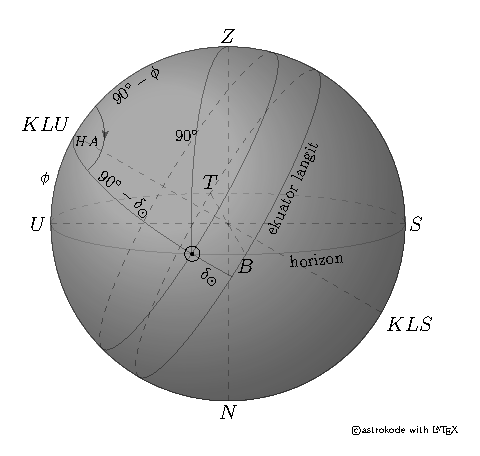
\includegraphics[scale=.655]{sunset.pdf}};  
\end{pgfonlayer}   

    \end{tikzpicture}
    \end{document}